% --------------------------------------------------------------------
% Preamble
% --------------------------------------------------------------------
\documentclass[a4paper, 12pt]{article} %Formato de plantilla que vamos a utilizar
\usepackage[utf8]{inputenc}
\usepackage[spanish]{babel}
\usepackage[a4paper, total={6.5in, 9.5in}]{geometry}
\usepackage{graphicx} % Insertar imagenes
\usepackage[table,xcdraw]{xcolor} % Deteccion de colores
\usepackage{fancyhdr} % Crear cabeceros
\usepackage{hyperref} % Enlances
\usepackage{listings} % Bloques de código

% --------------------------------------------------------------------
% Declaracion de colores
% --------------------------------------------------------------------
\definecolor{colorTitulo}{HTML}{0F52BA}
\definecolor{codegreen}{rgb}{0,0.6,0}
\definecolor{codegray}{rgb}{0.5,0.5,0.5}
\definecolor{codepurple}{rgb}{0.58,0,0.82}
\definecolor{backcolour}{rgb}{0.95,0.95,0.92}
\hypersetup{
  colorlinks,
  allcolors=.,
  urlcolor=blue,
}

% --------------------------------------------------------------------
% Declaracion de variables
% --------------------------------------------------------------------
\newcommand{\logoPunta}{img/LogoPuntaDelVerde.png} % Logo del punta
\newcommand{\logoKeter}{img/logo.png} % Logo de la practica
\newcommand{\nombrePractica}{Keter Vulnerability} % Nombre de la practica
\newcommand{\bigpar}{\par\vspace*{0.6cm}}
\newcommand\myfontsize{\fontsize{12pt}{14pt}\selectfont}


% --------------------------------------------------------------------
% Bloques de código
% --------------------------------------------------------------------
\lstdefinestyle{mystyle}{
    backgroundcolor=\color{backcolour},   
    commentstyle=\color{codegreen},
    keywordstyle=\color{magenta},
    numberstyle=\tiny\color{codegray},
    stringstyle=\color{codepurple},
    basicstyle=\ttfamily\footnotesize,
    breakatwhitespace=false,         
    breaklines=true,                 
    captionpos=b,                    
    keepspaces=true,                                  
    showspaces=false,                
    showstringspaces=false,
    showtabs=false,                  
    tabsize=2
}

\lstset{style=mystyle}

% --------------------------------------------------------------------
% Header y footer
% --------------------------------------------------------------------
\pagestyle{fancy}
\fancyhf{}
\rhead{\includegraphics[width=15cm]{\logoPunta}}
\rfoot{\textbf{Keter Vulnerability}\par Página \thepage}
\lfoot{\textbf{Emilio Sanchez Garcia}\par 2º ASIR}
\renewcommand{\headrulewidth}{0pt}
\renewcommand{\footrulewidth}{1pt}
\setlength\headheight{40.62811pt} % quitar aviso cabecero
\addtolength{\topmargin}{-0.62811pt}
\makeatletter							
\def\printauthor{				
    {\centering \large \@author}}				
\makeatother
\author{
		\textbf{Emilio Sánchez García}\\	
		IES Punta Del verde\\	
		Administración de Sistemas Informáticos en Red\\
        emilio.sanchez@outlook.es \\
}

% --------------------------------------------------------------------
% Comienzo del documento
% --------------------------------------------------------------------
\begin{document}
% Portada
\begin{titlepage}
	\centering
	\includegraphics[width=0.3\textwidth]{\logoKeter}\bigpar
	{\LARGE \textbf{Proyecto Final}\par\vspace{0.2cm}}
	{\Huge\bfseries\textcolor{colorTitulo}{\nombrePractica}}
	\vfill
	\printauthor
\end{titlepage}

% --------------------------------------------------------------------
% Indice
% --------------------------------------------------------------------
{\myfontsize \tableofcontents}

% --------------------------------------------------------------------
% Documentación
% --------------------------------------------------------------------
\newpage

% <----------- Introduccion ----------->
\vspace*{\fill}
\textcolor{colorTitulo}{\section{\Large Introducción}}
\vspace*{\fill}
\newpage

A día de hoy es extraño conocer una empresa que no tenga su propia web. Desde los inicios de Internet
todas empezaron a expandirse en este mundo tecnológico. Con el paso de los años, las apariciones de nuevas
técnicas las páginas web han ido incrementando su alcance. Desde mostrar únicamente un HTML plano hasta
tener multitud de funciones con otros servicios, y un trato de datos muy importante.\par
Conforme se fueron expandiendo, las empresas tuvieron que afrontar problemas nuevos. Sus web pasaron de
ser un expositor de información a contener datos realmente cruciales para las empresas. Los primeros
\textbf{hackers} aparecieron, haciendo un uso no pensado para la compañía. Esto les obligó a modificar
sus plataformas para poco a poco hacerlas más seguras, conforme se encontraban nuevos fallos.\bigpar

\begin{figure}[hbt]
	\centerline{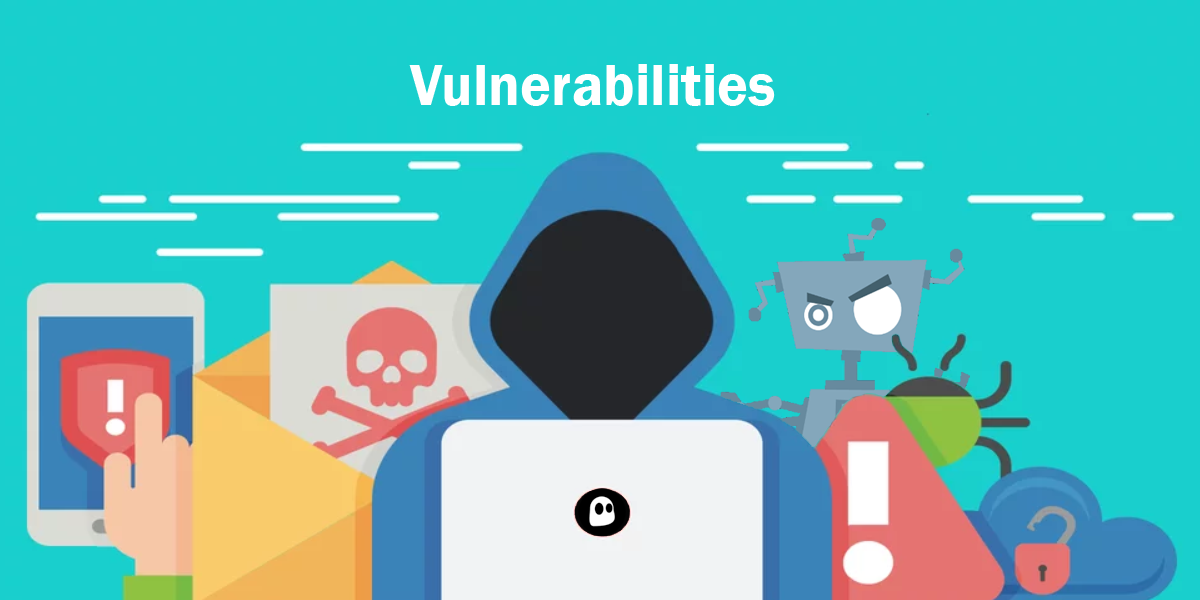
\includegraphics[width=1\textwidth]{img/vuln.png}}
	\caption[Vulnerability imagen]{Fuente \href{https://whiteknightit.com/2019/09/18/xeon-and-other-intel-cpus-hit-by-netcat-security-vulnerability/}{whiteknightit.com}}
\end{figure}

Esta palabra de \textbf{hacker} no debe tener la connotación negativa que tiene a día de hoy, gracias a
las películas. Un hacker es aquella persona que busca que un sistema informático funcione de una forma
distinta de la que está pensada. No necesariamente debe ir acompañado de robos de datos, extorsión,...\par
El hacker es aquel que busca vulnerabilidades en sistemas para explotarlas. Y esto ha conllevado a nuevos
trabajos en el entorno laboral. Uno de ellos es conocido como el \textbf{Bug Bounty Hunter}. Este trabajo
consiste en la búsqueda de estas vulnerabilidades, bien sea por errores en la configuración como fallos
nuevos, en sistemas en producción de empresas, siempre tratándose de entornos web.\par
Las empresas ofrecen sus páginas a estos hackers para que traten de vulnerarlas dentro de unas condiciones.
Compensando económicamente a aquellos que lo consigan.\bigpar
\newpage

\textbf{Keter Vulnerability} es una página web diseñada para representar fallas de seguridad a la hora
de crear aplicaciones web. El objetivo es disponer a los usuarios de diferentes \textbf{retos} donde
deberán usar sus conocimientos y sus herramientas.\par
Cada reto va acompañado de pequeñas pistas que ayudarán a los usuarios. Si bien no son pistas muy
explícitas, darán un punto de partida a la hora de buscar en Internet. Pues para el hacker, la herramienta
más importante es el propio navegador.\bigpar

\begin{figure}[hbt]
	\centerline{
\includegraphics[width=0.25\textwidth]{img/logo.png}}
	\caption[Vulnerability imagen]{Logo Keter Vulnerability}
\end{figure}

Se trata de ser capaces de concienciar a nuevos \textbf{desarrolladores} del peligro que puede
llevar realizar páginas web sin conciencia sobre sus fallos. Al final veremos como el usuario
es un factor bastante peligroso para ellos y como nunca podemos confiar plenamente en sus intenciones.\par
Muchos de estos errores se pueden ver como simples errores a la hora de plantear el funcionamiento de estos
sistemas. Otros en cambio serán algo más avanzados, utilizando vulnerabilidades comunes que se repiten
en multitud de páginas. Utilizaremos a la organización de \textbf{OWASP} (Open Web Application Security Project)
como mayor referente en este campo.\bigpar

\begin{figure}[hbt]
	\centerline{
\includegraphics[width=0.75\textwidth]{img/owasp-logo.png}}
	\caption[Vulnerability imagen]{Logo OWASP}
\end{figure}
\newpage

El objetivo de esta página es su \textbf{escabilidad}. No se busca que termine como está, sino que otros usuarios puedan aportar
sus propias ideas y retos, añadiendo nuevos a la página. Es por ello que se ha tomado la decisión usar todo el
lenguaje en inglés.\bigpar

Se hará uso de las últimas tecnologías para la realización de este proyecto:
\begin{itemize}
	\item \textbf{LaTex}: este lenguaje de edición de texto se utilizará para la creación de este mismo documento. LaTex
	      presenta un referente a la hora de la creación de informes, gracias a su poco peso y su fácil control.
	\item \textbf{NodeJS}: esta plataforma, de código abierto, servirá como base de este proyecto gracias a la gran
	      cantidad de herramientas que incorpora.
	\item \textbf{Mongo Atlas}: se utilizará una base de datos no relacional, en este caso MongoDB. Para tener una mayor
	      disponibilidad y no tener que depender de bases de datos internas utilizaremos su versión gratuita en la nube;
	      MongoAtlas.
	\item \textbf{GitHub}: la mayor página de código del mundo será donde se suba todo el proyecto, así como su avance
	      y otras guías, como la de su instalación.
	\item \textbf{Docker}: a modo de escabilidad de la página, se podrá usar Docker para hacer un rápido \textbf{deploy}
	      sin necesidad de montar la web en nuestra máquina anfitriona.
\end{itemize}
\begin{figure}[hbt]
	\centerline{
\includegraphics[width=0.16\textwidth]{img/latex.png}
		
\includegraphics[width=0.16\textwidth]{img/node.png}
		
\includegraphics[width=0.16\textwidth]{img/mongo.png}
		
\includegraphics[width=0.16\textwidth]{img/github.png}
		
\includegraphics[width=0.16\textwidth]{img/docker.png}}
\end{figure}
\clearpage

% <----------- Backend ----------->
\vspace*{\fill}
\textcolor{colorTitulo}{\section{\huge Backend}}
\vspace*{\fill}
\newpage

En el mundo del desarollo web se utilizan con frecuencia las conocidas API (Application Programming Interface). Estos
entornos sirven a menudo como pase intermedio de una aplicación web con una base de datos, protegiéndola así y
pudiendo dividir la carga de trabajo. Existen multitud de APIs públicas y privadas en Internet, pero en este caso
montaremos nuestra propia API en lo que se conoce como \textbf{Backend}, la parte que trabajo por detrás de la web.\bigpar

La API de esta aplicación contará con una sencilla base de datos en MongoDB. Se utilizarán tecnologías de la
\textbf{nube}, en concreto \textbf{MongoAtlas}, lo que permitirá su acceso desde cualquier web, siempre y cuando se
tengan las credenciales necesarias. El objetivo de esta base de datos no será tenerla protegida, por lo que le daremos
un tratamiento más flexible.
\newpage

\subsection{package.json}

Este archivo se crea automáticamente en proyectos \textbf{node.js}. Dicho archivo contiene toda la
información necesaria sobre el proyecto, en concreto sobre sus módulos y versiones instalados con \textbf{npm}.\par
Gracias a \textbf{package.json} se puede realizar el comando \textbf{npm install} a la hora de iniciar un proyecto
e instalará todos lo necesario para su funcionamiento.\bigpar

Así se verá el archivo con las librerías utilizadas:\par
\begin{figure}[hbt]
	\centerline{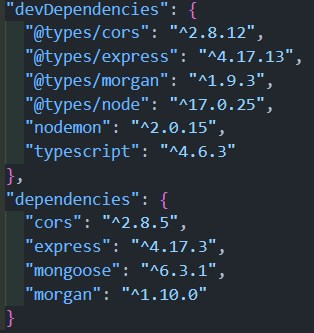
\includegraphics[width=0.4\textwidth]{img/api/zeropio-05184233.jpg}}
	\caption[Database]{package.json de la API.}
\end{figure}
\par
Estas librerías son:\par
\begin{itemize}
	\item \textbf{cors} (Cross-Origin Resource Sharing): esta librería permite que el proyecto sea accesible desde otros dominios, lo que le da la propiedad de API.
 \item \textbf{express}: ayudará en la comunicación \textbf{base de datos - API}.
 \item \textbf{mongoose}: esta librería servirá para implementar la integración de nuestra API con una base de datos MongoDB.
 \item \textbf{morgan}: actúa como \textbf{middleware}, añadiendo funciones necesarias como pueden ser \textbf{request}, \textbf{response},...
 \item \textbf{nodemon}: gracias a esta librería podremos lanzar nuestra API.
\end{itemize}

\newpage

\subsection{Conexión a la base de datos}
Con el siguiente archivo se realizará a la base de datos. Usaremos las credenciales \textbf{loginAccess:loginAccess}, que únicamente nos permitirá
leer la colección de \textbf{logins}.
El archivo se ve de la siguiente forma:
\begin{figure}[hbt]
	\centerline{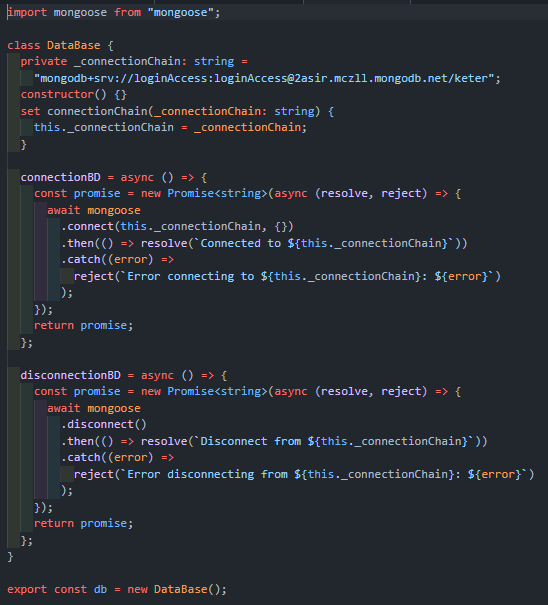
\includegraphics[width=0.9\textwidth]{img/api/04-12-44-33.png}}
	\caption[Database]{Archivo de conexión a MongoAtlas.}
\end{figure}
\clearpage

\subsection{Modelo}
Crearemos un modelo que será la pantilla que usará nuestra API para buscar documentos similares en la base de datos
y especificarle la colección a la que deberá apuntar.\par
\begin{figure}[hbt]
	\centerline{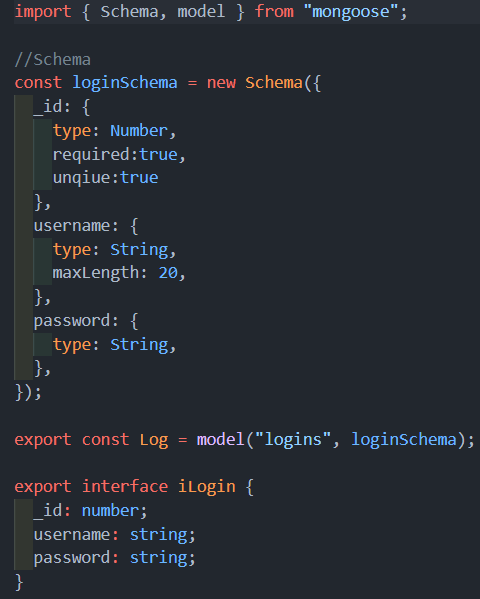
\includegraphics[width=0.65\textwidth]{img/api/04-12-45-52.png}}
	\caption[Model]{Modelo e interfaz de la colección.}
\end{figure}
\par
Usaremos limitadores de caracteres para el usuario y requeriremos el \textbf{ID}, para asegurarnos que todo es correcto.
Debido a que esta base de datos tan solo simula un caso real, las contraseñas viajarán en plano entre la API y
la web. En caso reales estas contraseñas se almacenarían cifradas y el ID no debería viajar nunca. Pero para
representar algunas de estas vulnerabilidades será necesario este \textbf{tratamiento de los datos}.
\newpage

\subsection{Rutas}
La parte más importante de la API son las \textbf{rutas}. Estas funciones nos permiten hacer las búsquedas en la base de datos,
sanear la entrada del usuario y filtrar valores modificando la URL con la que nos conectaremos a nuestra
API. En nuestro caso tendremos cinco rutas:
\begin{itemize}
	\item \textbf{Función de prueba}:
	      Esta función nos servirá únicamente para comprobar que la API está funcionando correctamente, pues tan solo devolverá un string.
	      \begin{figure}[hbt]
		      \centerline{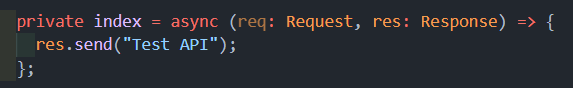
\includegraphics[width=0.8\textwidth]{img/api/04-12-46-08.png}}
		      \caption[Model]{Ruta de prueba.}
	      \end{figure}
	\item \textbf{Función de usuarios}:
	      Esta función tomará todos los usuarios y contraseñas de la base de datos y nos los devolverá al completo.
	      \begin{figure}[hbt]
		      \centerline{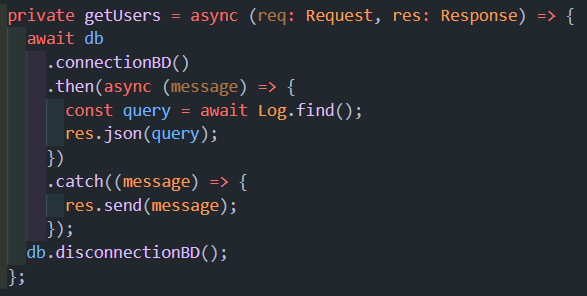
\includegraphics[width=0.8\textwidth]{img/api/04-12-46-13.png}}
		      \caption[Model]{Ruta de usuarios.}
	      \end{figure}
	      \newpage
	\item \textbf{Función de usuario}:
	      Esta función tomará el id de un usuario y mostrará sus datos.
	      \begin{figure}[hbt]
		      \centerline{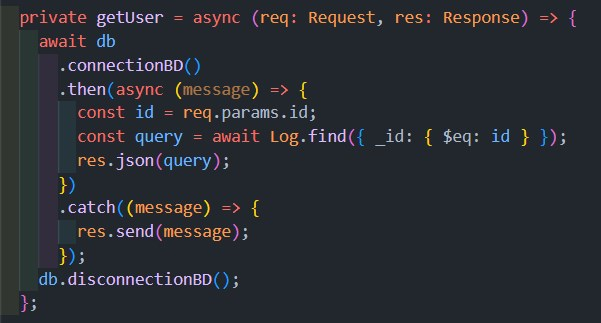
\includegraphics[width=0.8\textwidth]{img/api/zeropio-05132542.jpg}}
		      \caption[Model]{Ruta de usuarios.}
	      \end{figure}
	\item \textbf{Función de contraseña}:
	      Esta función tomará el nombre del usuario y devolerá su contraseña. Puede no ser una búsqueda
	      muy segura en entornos reales, pero será necesario para el proyecto y el funcionamiento de sus retos.
	      \begin{figure}[hbt]
		      \centerline{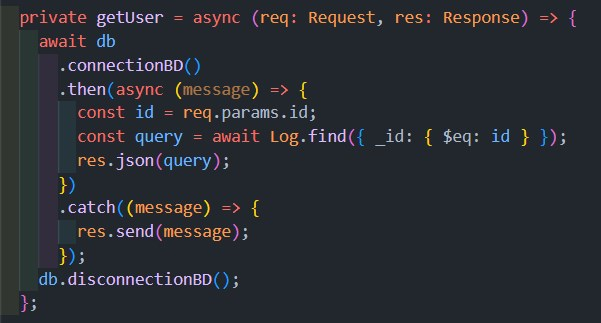
\includegraphics[width=0.8\textwidth]{img/api/zeropio-05132542.jpg}}
		      \caption[Model]{Ruta de usuarios.}
	      \end{figure}
	      \newpage
	\item \textbf{Función de login}:
	      Esta función será la más importante, ya que con ella haremos el login de la aplicación. Buscará dos valores que le enviaremos,
	      el usuario y su contraseña y comprobará que existen.
	      \begin{figure}[hbt]
		      \centerline{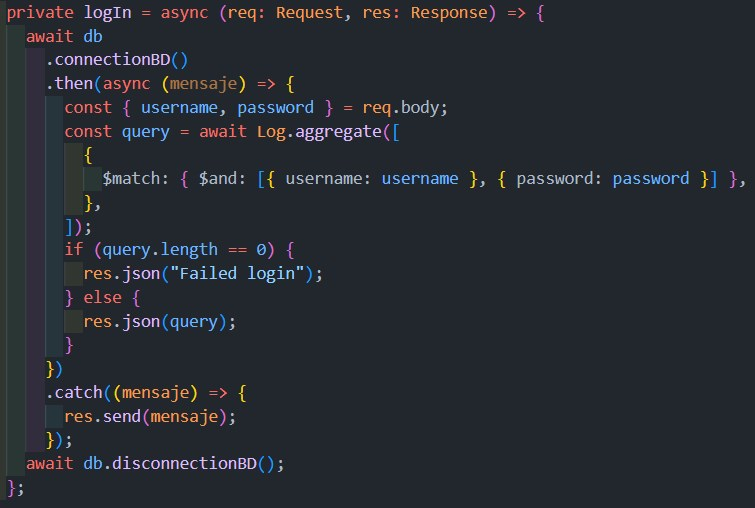
\includegraphics[width=1\textwidth]{img/api/zeropio-05132641.jpg}}
		      \caption[Model]{Ruta de login.}
	      \end{figure}
\end{itemize}
Finalmente deberemos declarar todas las rutas con su correspondiente método y dirección:
\begin{figure}[hbt]
	\centerline{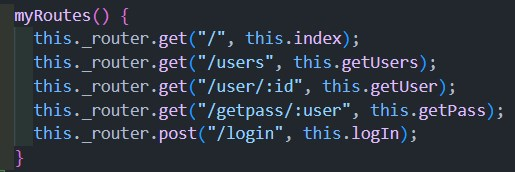
\includegraphics[width=0.65\textwidth]{img/api/zeropio-05132901.jpg}}
	\caption[Model]{Rutas.}
\end{figure}
\par
Utilizaremos el método \textbf{GET} cuando queramos obtener datos directamente desde la base de datos.
El método \textbf{POST} tendrá la misma función que el GET en nuestro caso, con una ligera diferencia. Los
datos enviados por POST se hacend desde el \textbf{body} de la web, al contrario de los GET que se hacen
desde la URL. Esto otorga una ligera capa extra de seguridad al no viajar los datos directamente.


\clearpage

% <----------- Frontend ----------->
\vspace*{\fill}
\textcolor{colorTitulo}{\section{\huge Frontend}}
\vspace*{\fill}
\newpage

El \textbf{frontend} es la parte contraria del backend. Mientras la anterior se encarga de las operaciones
que no están a la vista del usuario, como puede ser la comunicación \textbf{base de datos - servidor}, el
frontend se encarga de la parte visual para los usuarios. Cualquier página web que vemos es el frontend.\bigpar

Existen multitud de lenguajes de programación, y con casi todos se puede programar un frontend. Sin embargo,
los conocidos como \textbf{Framework} ayudan en este proceso. Estos framework son estructuras de un lenguaje de
programación concreto que cuentan con varias funciones propias. Esto ayuda a la hora de realizar aplicaciones, sean
del tipo que sean.\bigpar

La app de \textbf{Keter Vulnerability} utilizará el framework de \textbf{Angular}, uno de los más famosos y utilizados a
día de hoy junto a \textbf{React} o \textbf{Vue}. Angular utiliza el lenguaje de JavaScript, que se ejecuta en el lado del
cliente (a diferencia de otros lenguajes como \textbf{PHP} que se ejecutan en el lado del cliente).\par
Este proyecto no se realizará en JavaScript, se utilizará TypeScript que es un lenguaje derivado de JS.
Este lenguaje está altamente tipado, lo que ayuda a la hora de programar ya que cuenta con multitud de funciones.
Desde este lenguaje se compilará a JavaScript, que será el lenguaje que finalmente Angular comprenda.\bigpar

Para ayudarnos al diseño de la web añadiremos \textbf{Bootstrap}, una librería de CSS que dará formato. Y
\textbf{Angular Material}, que es otra librería de uso similar a Bootstrap, pero creada por y para Angular.
\newpage

\subsection{package.json}

Al igual que en el backend, este apartado creará su propio archivo igualmente.\bigpar

Así se verá el del proyecto archivo:\par
\begin{figure}[hbt]
	\centerline{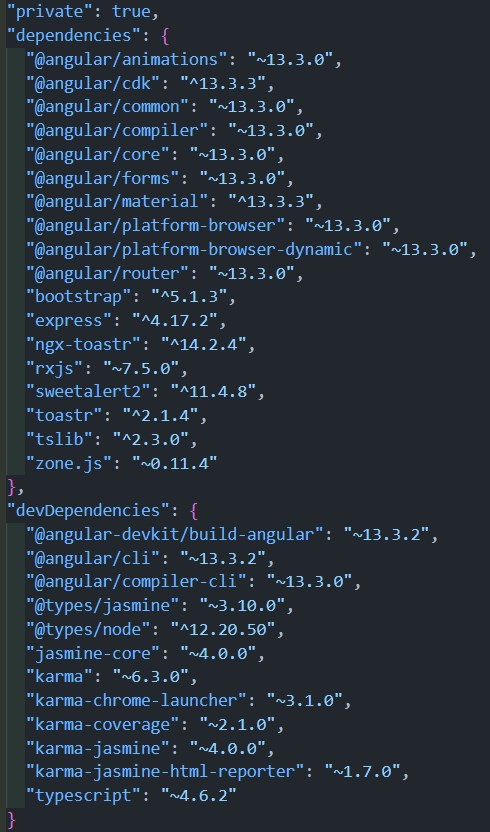
\includegraphics[width=0.55\textwidth]{img/app/zeropio-05182859.jpg}}
	\caption[Rutas]{package.json de la App.}
\end{figure}
\newpage
Estos serán:\par
\begin{itemize}
	\item \textbf{bootstrap}: como ya se ha mencionado anteriormente, esta librería aportará estilos nuevos.
	\item \textbf{Angular Material}: al igual que Bootstrap, esta librería nos dará nuevos estilso.
 \item \textbf{express}: es un frameworkd de Node.js que servirá en la comunicación \textbf{backend - frontend}.
 \item \textbf{ngx-toastr} y \textbf{toastr}: será uno de los modulos que añadan notificaciones dentro de la web.
 \item \textbf{rxjs}: esta librería añadirá funciones para conversaciones con la API que utilicen \textbf{observables}.
 \item \textbf{sweetalert2}: al igual que ngx-toastr nos aportará notificaciones.
 \item \textbf{tslib}: nos ofrece comandos de ayuda para programación en TypeScript.
 \item \textbf{zone.js}: añade funciones asíncronas.
\end{itemize}

\newpage

\subsection{Rutas}
Para poder tener una mayor optimización se han separado las distintas rutas, de esta forma tan solo cargarán
unas páginas dependiendo de en que parte de la aplicación se encuentre.\par
\begin{figure}[hbt]
	\centerline{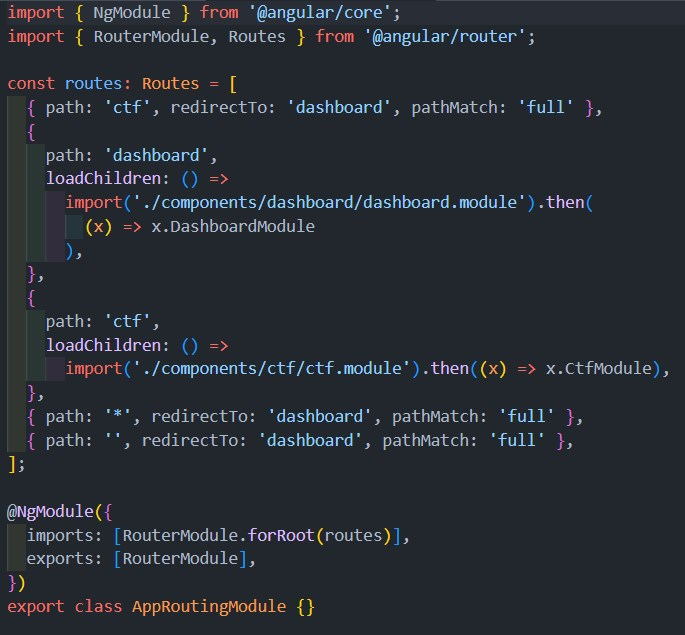
\includegraphics[width=0.8\textwidth]{img/app/zeropio-05181221.jpg}}
	\caption[Rutas]{rutas principales.}
\end{figure}
\par
Estas rutas son las primeras, se encuentran en el archivo por defecto creado por Angular.\par
La primera declaración redirige al \textbf{dashboard} cualquier ruta vacia. La segunda redirige la ruta
\textbf{ctf} al dashboard igualmente.
La siguiente ruta es la del dashboard, en vez de cargar entero el dashboard y todos sus componentes cargamos
únicamente la propia página, de igual manera que hacemos con el \textbf{ctf}.\newpage
Veremos a continuación las rutas del dashboard:\par
\begin{figure}[hbt]
	\centerline{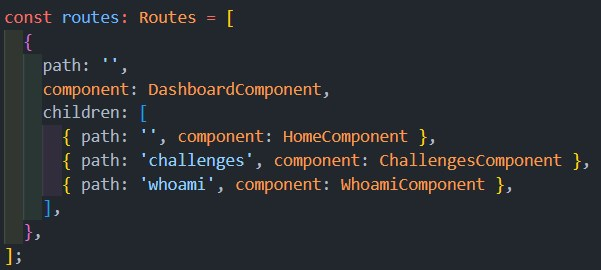
\includegraphics[width=0.6\textwidth]{img/app/zeropio-05181636.jpg}}
	\caption[Rutas]{rutas hijas del Dashboard.}
\end{figure}
Estas rutas son cargadas únicamente cuando se ingresa al Dashboard. De esta forma podemos tener la app
dividida en dos partes. Por otro lado el \textbf{ctf} tiene su propio archivo de rutas del que parten los demás
componentes, esto nos permite ahorrar la carga de todos los retos cuando tan solo hemos entrado al Dashboard.
De igual manera, mientras nos encontremos en un reto no tendremos el Dashboard cargando también.\bigpar

Estas serán las rutas de los retos:\par
\begin{figure}[hbt]
	\centerline{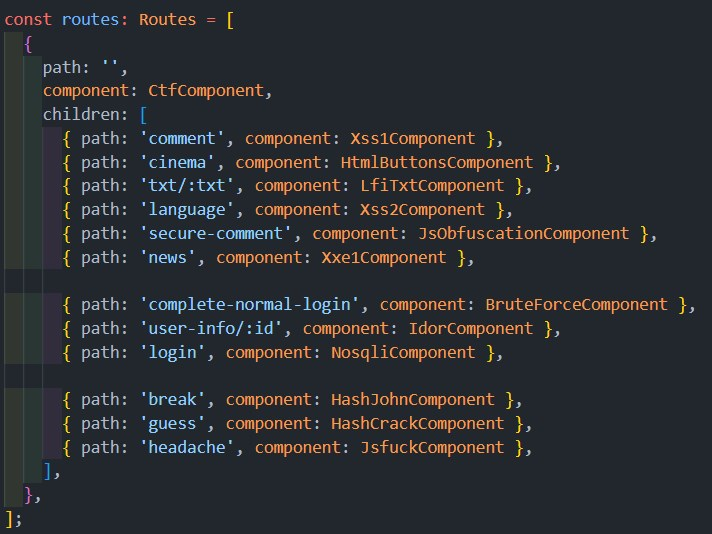
\includegraphics[width=0.75\textwidth]{img/app/zeropio-05181728.jpg}}
	\caption[Rutas]{rutas hijas del CTF.}
\end{figure}
\par
Algunas de estas rutas aceptarán un parámetro (la sintaxis es \textbf{:texto}), ya que será necesario para dicho reto.
\newpage

\subsection{Módulos}
Hemos separado también los módulos para una carga más rápida. Mantenemos el archivo por defecto de los módulos
pero importamos un nuevo módulo que hemos creado nosotros: \textbf{Shared}.\par
\begin{figure}[hbt]
	\centerline{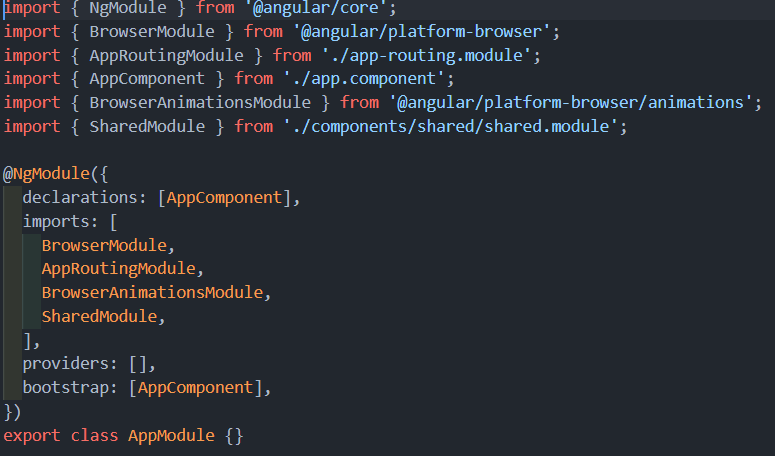
\includegraphics[width=0.9\textwidth]{img/app/15-17-53-17.png}}
	\caption[Modulos]{\textbf{app.module.ts} por defecto.}
\end{figure}
En dicho módulo \textbf{Shared} importamos todos los módulos que usamos para el proyecto, de esta forma podemos dividir
los archivos y tener un mayor control de errores.\par
Al finalizar el proyecto se puede ver como se han tenido que implementar una gran cantidad de
módulos:\par
\begin{figure}[hbt]
	\centerline{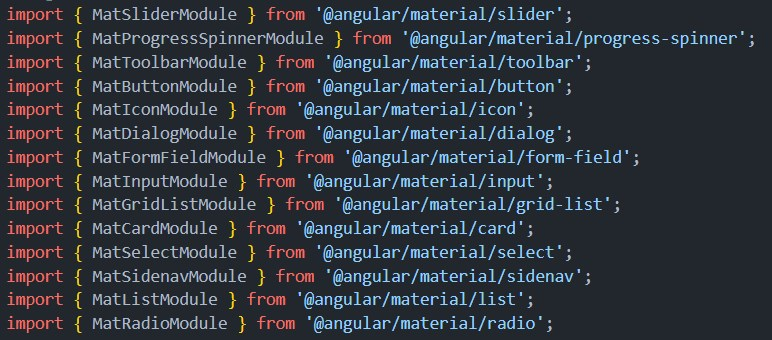
\includegraphics[width=0.9\textwidth]{img/app/zeropio-05182101.jpg}}
	\caption[Modulos]{\textbf{app.module.ts} finalizado.}
\end{figure}
\newpage

\subsection{DOMsanitizer}
Angular por defecto viene protegido contra ciertas vulnerabilidades, para poder recrearlas ha sido necesario escapar
algunos de estas protecciones, como por ejemplo \textbf{DOMsanitizer}.\par
\begin{figure}[hbt]
	\centerline{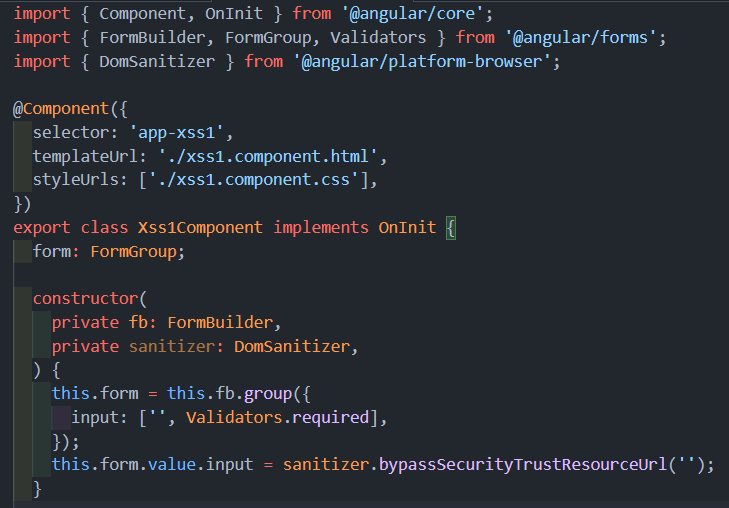
\includegraphics[width=1\textwidth]{img/app/15-18-06-57.png}}
	\caption[Modulos]{desactivar DOMsanitizer.}
\end{figure}
\par
Para poder escapar la seguridad lo primero que se hará será usar los formularios de Angular para poder
tomar el valor en una variable. Se importará la librería de DOMsanitizer y establecerá el valor
como fiable, de esta forma se podrá explotar algunas vulnerabilidades, como \textbf{XSS}.
\clearpage


% <----------- Vulnerabilidades ----------->
\vspace*{\fill}
\textcolor{colorTitulo}{\section{\huge Vulnerabilidades}}
\vspace*{\fill}
\newpage

\subsection{Código inseguro}
Con esta vulnerabilidad nos referimos a código que se ejecuta en la parte del cliente y se confía en su fiabilidad. Esto puede ser
por ejemplo, un botón desactivado ya que lleva a una función que no tenemos habilitada. Pero en lugar de desactivar esa función,
simplemente dejamos el botón del lado del cliente como \textbf{disable}.\par
Esto puede llevar a que un usuario simplemente modifique el código, active nuevamente el botón y acceda a partes no deseadas.
\bigpar

\subsection{Cross Site Scripting}
Cross-Site Scripting (\textbf{XSS}) son un tipo de ataque mediante inyección, mediante el cual código malicioso es inyectado
en páginas confiables. Los ataques de XSS ocurren cuando el atacante usa una aplicación web para enviar
código malicioso, generalmente en forma de script de navegador, para un tercer usuario. Puede ocurrir en multitud
de aplicaciones web mediante la entrada de un usuario, sin validar o codificar su valor.\par
\begin{footnotesize}
	Fuente: \href{https://owasp.org/www-community/attacks/xss/}{OWASP Cross Site Scripting (XSS)}
\end{footnotesize}
\bigpar
Existen principalmente tres tipos de XSS, estos son:
\begin{itemize}
	\item \textbf{Reflected}: es el más común de los tres. Ocurre cuando la aplicación recibe datos en una petición \textbf{HTTP}
	      y lo incluye directamente.
	\item \textbf{Stored}: este tipo es el más peligroso, ya que los datos se quedan guardados en una parte visible de la aplicación. Esto
	      significa que cualquiera que acceda a esa página, como puede ser un comentario, se verá afectado.
	\item \textbf{DOM}: este tipo es el presente en la URL. Su peligro llega cuando esa misma dirección URL se puede enviar a otros usuarios,
	      pudiendo parecer una aplicación segura al venir de una fuente confiable, sin que sepamos que estamos siendo afectados.
\end{itemize}

Existen múltiples formas de realizar un XSS y múltiples formas de bloquearlo. Lo más común es encontrar filtros que rompan ciertos caracteres, como
pueden ser los \textbf{<>} o palabras como \textbf{script}. De la misma forma que surgen estos bloqueos, surge la parte contraria encargada de saltarse
(\textbf{bypass}) estas medidas de seguridad.\par
A menudo, suele ser mediante codificación del código. Usando caracteres especiales como \textbf{\textbackslash} o convirtiendo al texto en hexadecimal se
pueden saltar algunos de los filtros más sencillos.

\newpage

\subsection{Local File Inclusion}
Ciertas aplicaciones web leen archivos locales que puedan tener almacenados en su servidor. A simple vista esto no presenta ningún problema,
pero si la configuración no ha sido correcta el usuario podría modificar la búsqueda de ruta de dicho archivo para moverse a
través del sistema.\par
Esta vulnerabilidad, conocida como \textbf{LFI}, nos permite recopilar información importante sobre el sistema y hasta ejecutar
código. La forma más típica de vulnerarla es cambiar la url del archivo por un salto hacia atrás de muchos directorios
(\textbf{../../../../}), esto nos permitirá acceder a la raíz. En sistemas \textbf{Linux}, añadiendo un \textbf{/etc/passwd} al
final de la URL nos permitirá listar todos los usuarios del sistema.\bigpar

El problema llega con el \textbf{Log Poisoning}, donde podemos añadir líneas a logs y luego visualizarlos para ejecutar código.
Por ejemplo, si tratamos de logearnos mediante \textbf{SSH} con un usuario como: \textbf{nc -e /bin/bash 127.0.0.1:443}, se
guardará ese registro en el log (dicho código es una \textbf{reverse shell}).\par
Si ahora usaramos el LFI para llegar hasta dicho log, se ejecutará el código que hemos incluido, ganando acceso al sistema.

\subsection{XML External Entity Injection}
XML External Entity Injection (\textbf{XXE}) es una vulnerabilidad similar que ocurre en archivos XML. En múltiples web donde es posible
subir archivos, o texto, en formato XML se puede llegar a inyectar código si el texto no esta sanizado.\par
A menudo, estos archivos de XML que piden las páginas solicitan que contengan ciertos campos, pero XML nos permite crear ciertas funciones
como comandos que se ejecuten. Algo como lo siguiente podría ejecutar código en el sistema:
\begin{lstlisting}
<?xml  version="1.0" encoding="utf-8"?>
<!DOCTYPE replace [<!ENTITY xxe SYSTEM  "file:///etc/passwd" >]>
<author>&xxe;</author>
\end{lstlisting}

\subsection{NoSQL Injection}
Una de las vulnerabilidades más conocidas es \textbf{SQLi} o \textbf{SQL Injection}. Dicha vulnerabilidad suele ocurrir en los
inicios de sesión. Si la petición para iniciar sesión es mediante una \textbf{query} de SQL que acepta la entrada del usuario
directamente, el atacante podría modificar dicha query añadiendo código, por ejemplo: \textbf{' -- \#}.
\bigpar
Pero esto no solo ocurre en bases de datos relacionales, también puede ocurrir en las no relaciones, como es el caso de Mongo.\par
La sintaxis es sencilla, simplemente debemos modificar uno de los dos parámetros (usuario o contraseña) para ganar acceso a cuentas
que no deberíamos.\par
Existen muchos tipos, dependiendo si la aplicación devuelve errores o no, que tipo de query usa e incluso si sanea la entrada del
usuario. A veces estas sanaciones son demasiado cortas, usando por ejemplo listas negras de palabras, que se pueden saltar fácilmente.

\subsection{Ataques a contraseñas}
Una de las técnicas más comunes es el ataque a contraseñas. Suele aparecer en logins, aunque no siempre tiene porqué. Consiste en la repetición de
intentos de inicio de sesión, probando múltiples posibles contraseñas. A menudo esta técnica se suele emplear mediante programas de automatización
que ingresan las contraseñas. Puede haber varios casos, como son:
\begin{itemize}
	\item \textbf{Por diccionario}: utilizan conjuntos de palabras. A menudo estos diccionarios ya han sido escritos, como puede ser el caso del
	      famoso \textbf{rockyou.txt} o pueden ser creados por el atacante, bien a mano o mediante herramientas como \textbf{crunch}.
	\item \textbf{Fuerza bruta}: en vez de usar listas prueban múltiples combinaciones aleatorias que van generando.
\end{itemize}

\subsection{IDOR}
El \textbf{Insecure Direct Object References} (IDOR) nos permite modificar las peticiones de las páginas web. Por ejemplo,
cuando una URL hace una petición \textbf{/?s=...}, la página nos devuelve ciertos datos. Si modificamos este campo podemos tener acceso a
otras partes de la web que en las que no se ha considerado que debamos tener acceso.


\clearpage


% <----------- Explotaciones ----------->
\vspace*{\fill}
\textcolor{colorTitulo}{\section{\huge Explotaciones}}
\vspace*{\fill}
\newpage

\subsection{Send a comment!}
\begin{figure}[hbt]
	\centerline{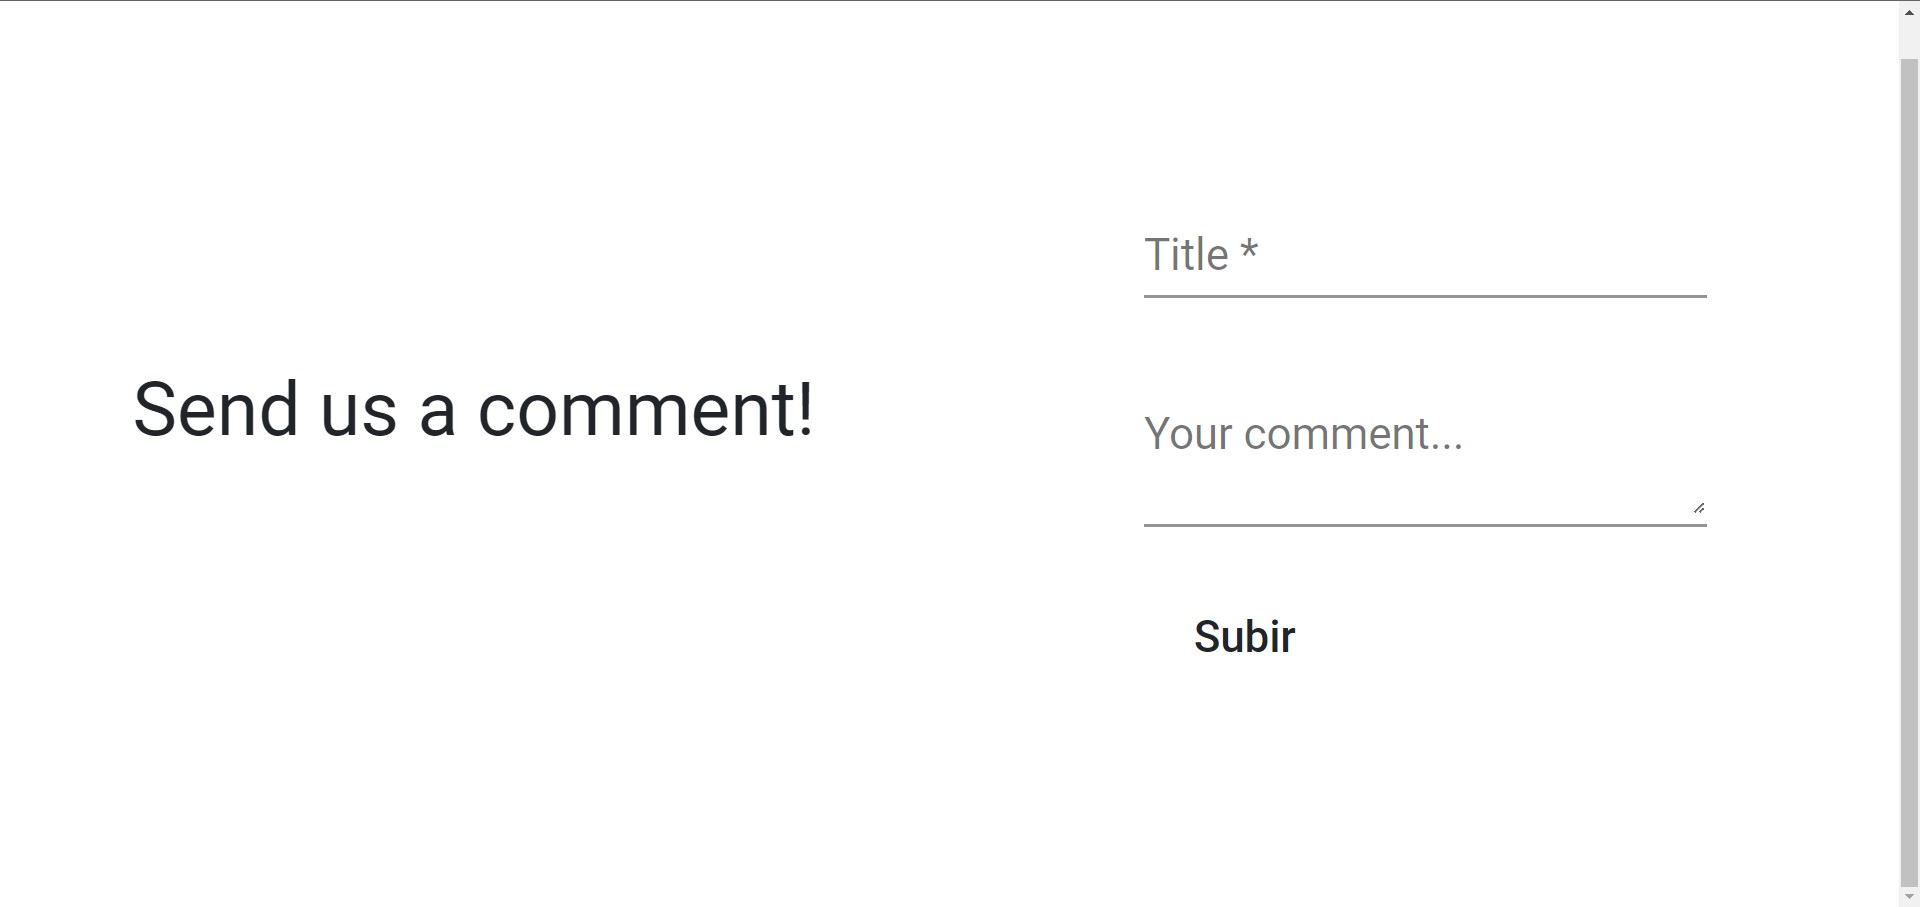
\includegraphics[width=0.75\textwidth]{img/ctf/zeropio-04183903.jpg}}
	\caption[Modulos]{Reto 1.}
\end{figure}
La explotación de este reto consiste en utilizar la vulnerabilidad de XSS Reflected.\par
Con tan solo poner un comando entre las etiquetas $<script>...</script>$ nos dará por solucionado
el reto.

\subsection{One ticket for Batman}
\begin{figure}[hbt]
	\centerline{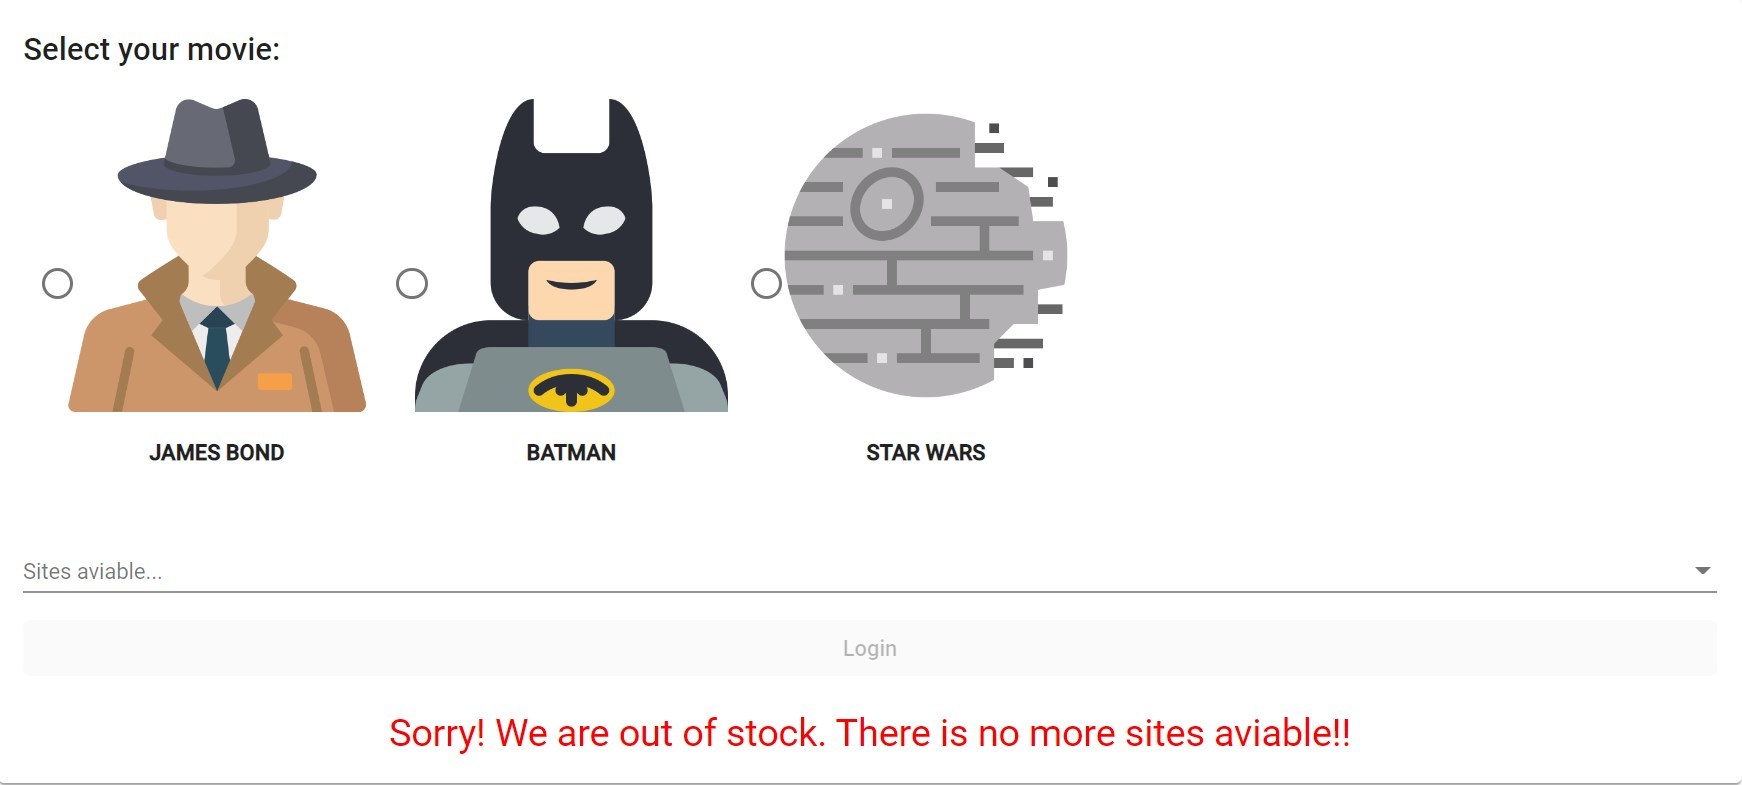
\includegraphics[width=0.75\textwidth]{img/ctf/zeropio-04183925.jpg}}
	\caption[Modulos]{Reto 2.}
\end{figure}
Esta vulnerabilidad es de las más sencillas. No podremos hacer nuestra reserva de una entrada ya que el botón HTML se encuentra
desactivado. Inspeccionando el código podremos volver a activarlo y reservar nuestra entrada sin problema.
\newpage

\subsection{This txt}
\begin{figure}[hbt]
	\centerline{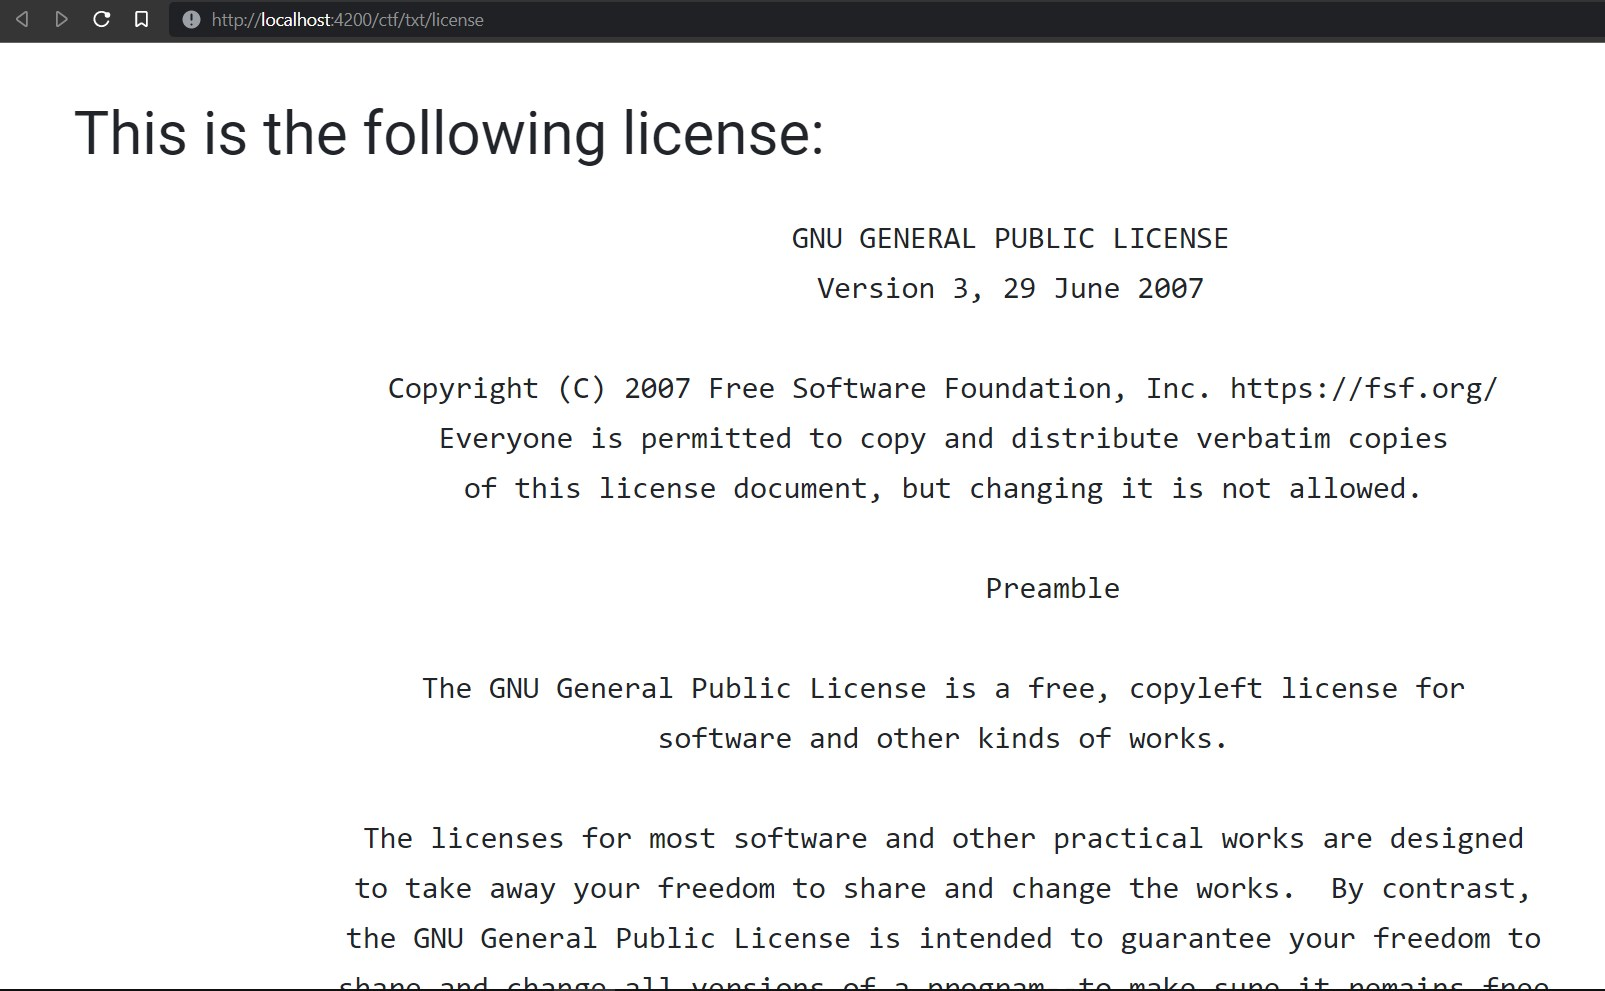
\includegraphics[width=0.75\textwidth]{img/ctf/zeropio-04184006.jpg}}
	\caption[Modulos]{Reto 3.}
\end{figure}
La explotación de este reto consiste en utilizar la vulnerabilidad de LFI.\par
Si miramos la URL veremos que está leyendo un archivo llamado \textbf{license}. La consola de la aplicación nos dará una pequeña
pista, diciendo que ya nos encontramos en la localización de \textbf{/etc}, por lo que modificando \textbf{license} por
\textbf{passwd} nos dará por completado el reto.

\subsection{Where are u from?}
\begin{figure}[hbt]
	\centerline{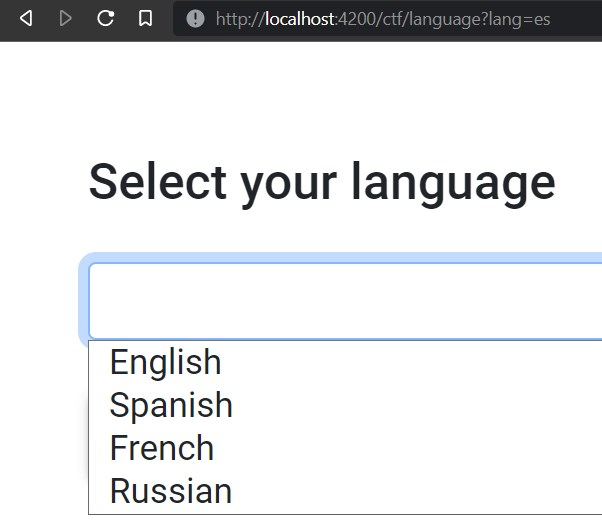
\includegraphics[width=0.3\textwidth]{img/ctf/zeropio-04184029.jpg}}
	\caption[Modulos]{Reto 4.}
\end{figure}
Para este reto usaremos el tipo de XSS DOM, esta vez tendremos una lista de opciones que elegir, por lo
que no podremos escribir el código en la página como antes. Sin embargo, podemos ver como en la URL aparece
la opción que hemos elegido.\par
Si probamos a escribir allí la misma sintaxis que el anterior ($<script>...</script>$) la página nos
impidirá introducir el script. Podemos probar otras sintaxis similares, como $javascript:...$, lo
cual sí funcionará.
\newpage

\subsection{Suscribe now!}
\begin{figure}[hbt]
	\centerline{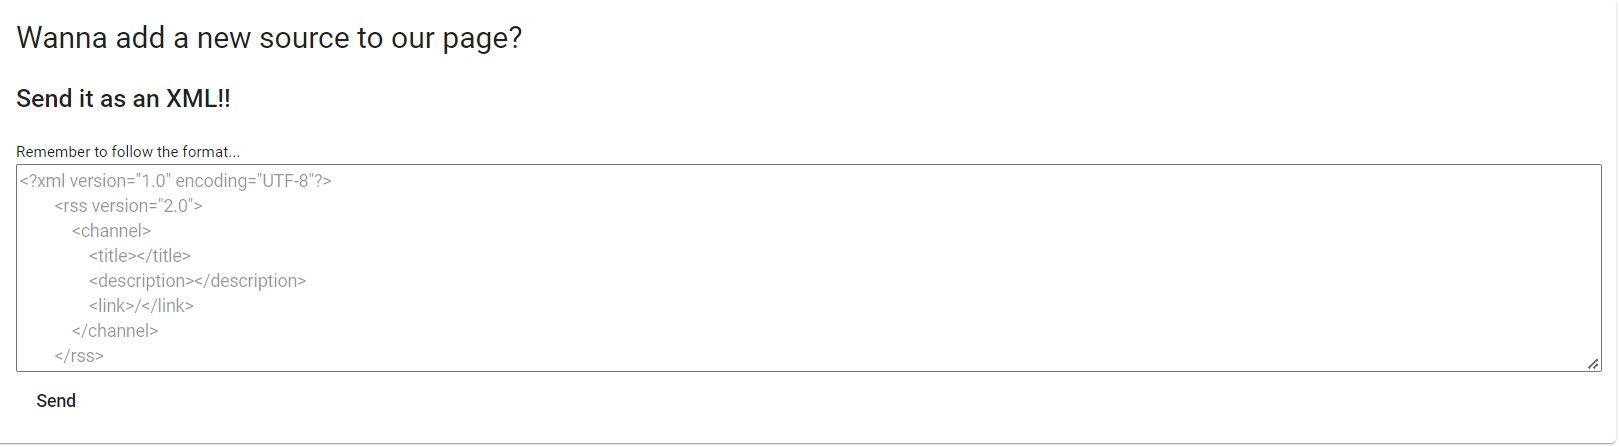
\includegraphics[width=0.9\textwidth]{img/ctf/zeropio-04184043.jpg}}
	\caption[Modulos]{Reto 5.}
\end{figure}
Este reto trata de un XXE. Se nos muestra un textarea donde debemos subir un XML con contenido de un periódico
para enlazarlo a la web. En cambio si tratamos de hacer un simple XXE donde podamos ejecutar código, como en el ejemplo
de arriba, nos dará por completado el reto.

\subsection{Not that easy}
\begin{figure}[hbt]
	\centerline{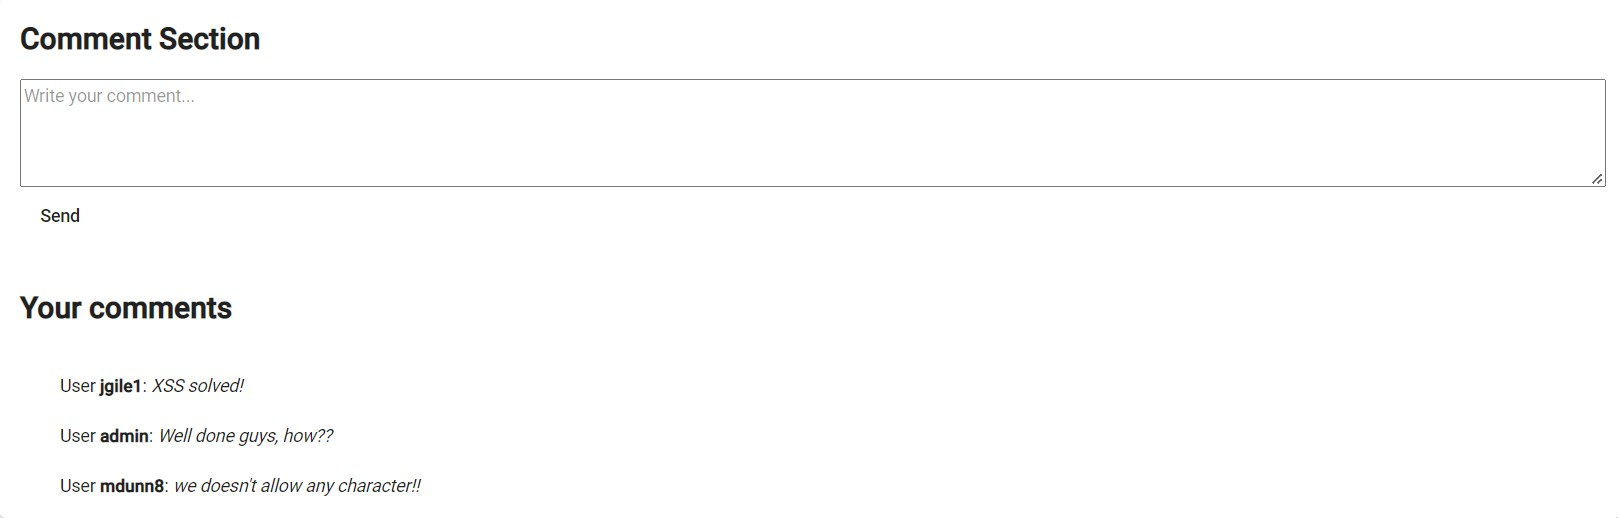
\includegraphics[width=0.9\textwidth]{img/ctf/zeropio-04184050.jpg}}
	\caption[Modulos]{Reto 6.}
\end{figure}
Se trata de un XSS stored donde podremos subir un comentario. Los comentarios de los anteriores usuarios nos dicen que los caracteres
son escapados, por lo que no podremos ejecutar código con etiquetas \textbf{script}.\par
Si codificamos el código con \textbf{jsFuck} nos dará el reto por resuelto.
\newpage

\subsection{Welcome user number one}
\begin{figure}[hbt]
	\centerline{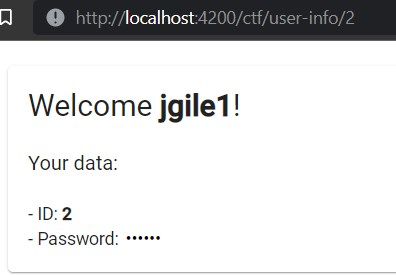
\includegraphics[width=0.3\textwidth]{img/ctf/zeropio-04184136.jpg}}
	\caption[Modulos]{Reto 7.}
\end{figure}
Este reto consistirá en un sencillo IDOR. Veremos que la URL lista al usuario con ID 2. Si vamos subiendo este número veremos la información de otros usuarios,
si nos dirigimos al usuario de ID 1, el admin, nos dará por resuelto el reto.

\subsection{Can you guess it?}
\begin{figure}[hbt]
	\centerline{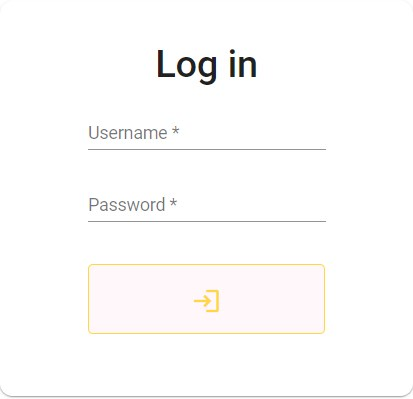
\includegraphics[width=0.4\textwidth]{img/ctf/zeropio-04184142.jpg}}
	\caption[Modulos]{Reto 8.}
\end{figure}
Se nos muestra un login nada más entrar al reto. En la consola podemos ver como se mencionan a dos usuarios, con un aviso de que deben cambiar
sus contraseñas. Cada usuario tendrá una resolución distinta.\par

Para el usuario \textbf{mdunn8} deberemos hacer uso de la herramienta \textbf{crunch}.
\begin{lstlisting}
> crunch 1 6 1234567890 -o wordlist.txt
\end{lstlisting}
Este comando generará secuencas de caracteres de mínimo \textbf{1} carácter y máximo \textbf{6}, que contengan \textbf{1234567890},
y los redigirán al archivo \textbf{wordlist.txt}.\par
Podremos usar este diccionario para ir probando las contraseñas con dicho usuario.\bigpar

Para el usuario \textbf{jgile1} usaremos un diccionario ya creado, como es el caso de \textbf{rockyou.txt}, el cual se encuentra en el propio Kali.\par

Para ambos usuarios, vamos a hacer uso de \textbf{BurpSuite}. Instalaremos en nuestro navegador la extensión \textbf{FoxyProxy}, que nos permite
tener diferentes configuraciones de proxy para poder cambiar rápidamente entre ellas.
\begin{figure}[hbt]
	\centerline{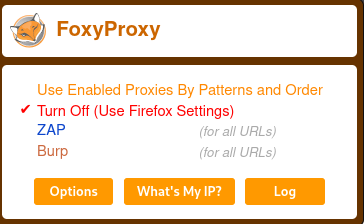
\includegraphics[width=0.3\textwidth]{img/app/15-16-26-07.png}}
	\caption[Modulos]{FoxyProxy.}
\end{figure}
Captaremos la request de la página con Burp, para ello nuestro proxy estará configurado como \textbf{127.0.0.1:8080}.\par
Una vez capturada en el apartado de \textbf{Proxy} lo enviaremos al \textbf{Intruder}, allí podremos elegir el valor de contraseña a repetir,
añadiéndolo entre dos \$.\par
En el Intruder elegiremos nuestros dos diccionarios creados anteriormente y los elegiremos, correremos la fuerza bruta mientras esperamos a que funcione.
\begin{figure}[hbt]
	\centerline{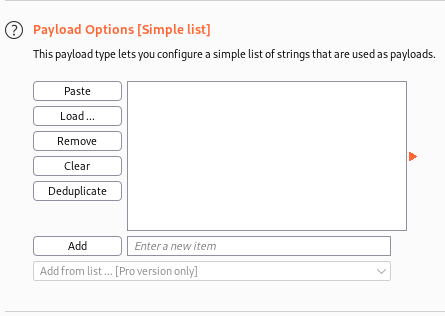
\includegraphics[width=0.75\textwidth]{img/app/15-16-29-47.png}}
	\caption[Modulos]{Burp Intruder.}
\end{figure}
\newpage

\subsection{Give me your password}
\begin{figure}[hbt]
	\centerline{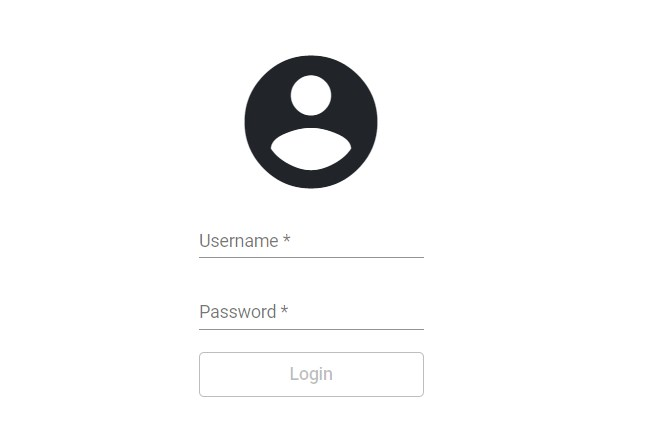
\includegraphics[width=0.75\textwidth]{img/ctf/zeropio-04184213.jpg}}
	\caption[Modulos]{Reto 9.}
\end{figure}
Este reto nos mostrará un login. Podemos loguearnos como el usuario test:test, pero para completar el reto
trataremos de entrar como admin, sabemos que está corriendo una base de datos MongoDB, por lo que podemos tratar de realizar un NoSQLi.\par
Usaremos una sintaxis sencilla de NoSQLi, como $"\$ne": 1$. Esto nos logueará como admin.

\subsection{Guess it...}
\begin{figure}[hbt]
	\centerline{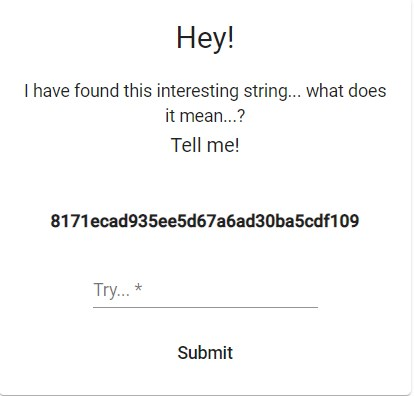
\includegraphics[width=0.35\textwidth]{img/ctf/zeropio-04184222.jpg}}
	\caption[Modulos]{Reto 10.}
\end{figure}
Este reto nos propondrá un hash que deberemos descifrar.\par
Con una simple búsqueda en Google podemos encontrar la solución a este reto.
\newpage

\subsection{Break it!}
\begin{figure}[hbt]
	\centerline{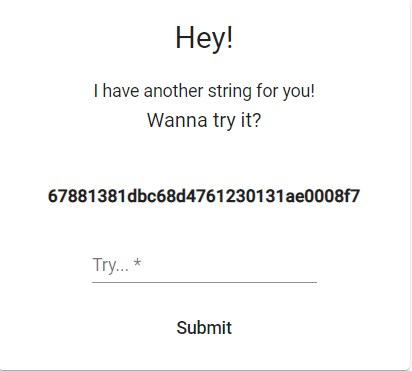
\includegraphics[width=0.35\textwidth]{img/ctf/zeropio-04184226.jpg}}
	\caption[Modulos]{Reto 11.}
\end{figure}
Este reto va un paso más adelante que el anterior. En vez de buscar el hash por internet deberemos
hacer uso de la herramienta \textbf{John The Ripper}. Con el siguiente comando podremos romperlo:
\begin{lstlisting}
> john --format=raw-md5 --wordlist=/usr/share/wordlists/rockyou.txt hash
\end{lstlisting}\bigpar
Como podemos ver:
\begin{figure}[hbt]
	\centerline{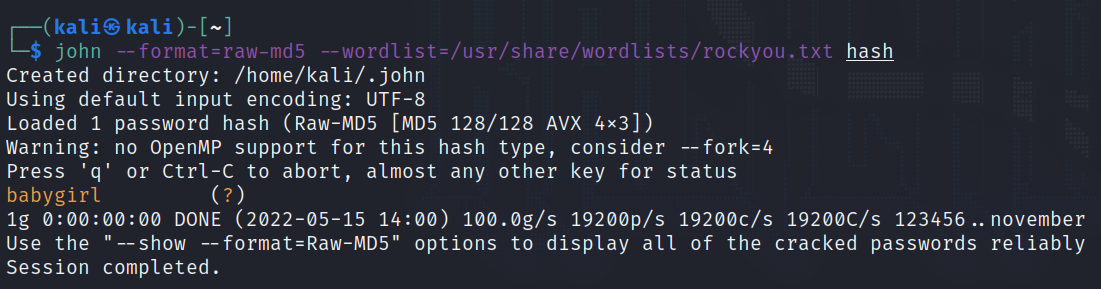
\includegraphics[width=0.75\textwidth]{img/app/15-20-00-30.png}}
	\caption[Modulos]{John rompiendo un hash.}
\end{figure}\par
John es capaz de romperlo, siempre y cuando usemos una wordlist que contenga el hash.
\newpage

\subsection{What is this?}
\begin{figure}[hbt]
	\centerline{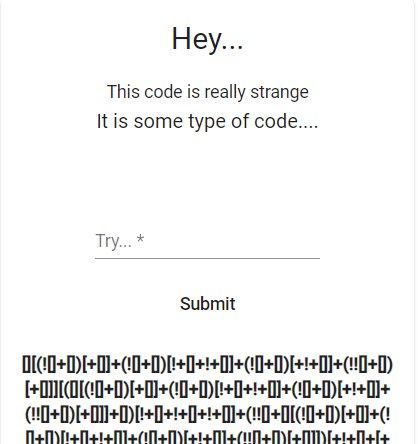
\includegraphics[width=0.35\textwidth]{img/ctf/zeropio-04184231.jpg}}
	\caption[Modulos]{Reto 12.}
\end{figure}
Volveremos a encontrarnos con código de jsFuck, si lo pasamos por un decoder encontraremos la solución.

\bigpar

\clearpage


% <----------- Posibles soluciones ----------->
\vspace*{\fill}
\textcolor{colorTitulo}{\section{\huge Posibles soluciones}}
\vspace*{\fill}
\newpage

\subsection{Código inseguro}
Esta solución requiere que no solo se tome en cuenta la parte del cliente, sino también la del servidor. Si queremos deshabilitar
una función no solo deberemos deshabilitar el botón que nos lleve a ella. También deberemos o eliminar temporalmente dicha parte
o añadirle un \textbf{error 403}.\par
En caso de aplicaciones que se conecten directamente con una API, como puede ser un \textbf{CRUD}, debemos asegurarnos que el
usuario no puede modificarlo desde la API.
\bigpar

\subsection{Cross Site Scripting}
Para esta vulnerabilidad la solución consiste en depurar la entrada del usuario. En vez de usar
DOMsanitizer para desactivarlo, si no lo nombramos por defecto estaría activado. Por asegurarnos podemos
especificar que depure esa parte. Para ello debemos usar la siguiente estructura:
\begin{lstlisting}
this.form.value.input = sanitizer.sanitize('');
\end{lstlisting}
en sustitución del código que teniamos anteriormente:
\begin{lstlisting}
this.form.value.input = sanitizer.bypassSecurityTrustResourceUrl('');
\end{lstlisting}
\begin{footnotesize}
	\textbf{Nota:} DOMsanitizer tiene distintos formatos y funciones, no se limita únicamente a estas dos, por lo que
	en algunos casos puede ser mejor utilizar otras.
\end{footnotesize}
\bigpar

\subsection{Local File Inclusion}
La forma más sencilla es cerrar a la aplicación. Tan solo le permitimos moverse entre ciertos directorios, por lo que nadie
podrá moverse transversalmente. Otra solución sería permitir tan solo que se vean ciertos ficheros que deseemos mediante una
lista blanca.\par
Pero para evitar esta vulnerabilidad en su totalidad la mejor solución es no leer ningún archivo del sistema.
\bigpar

\subsection{NoSQL Injection}
La solución para \textbf{NoSQLi} es la misma que para XSS y la norma principal en aplicaciones web. No confiar nunca en la entrada
del usuario. Los datos que introduzca deben ser tratados únicamente como string, sin permitir caracteres especiales.\par
Es buena práctica encriptarlo y desencriptarlo para evitar posibles \textbf{bypass} mediante encriptaciones del atacante.

\subsection{Ataques a contraseñas}
La forma más sencilla de protegerse contra estos ataques es:
\begin{itemize}
	\item Bloquear el número de intentos.
	\item Evitar usar contraseñas sencillas o que puedan aparecer en bases de datos de contraseñas filtradas.
\end{itemize}

\subsection{IDOR}
La protección contra IDOR más sencilla es evitar usar búsquedas GET en la url.
Pero otra forma es tener bien controlado que páginas se tiene permiso de acceso y cuales no, independientemente de si están
indexadas o no.

\clearpage


% <----------- Introduccion ----------->
\vspace*{\fill}
\textcolor{colorTitulo}{\section{\huge Conclusión}}
\vspace*{\fill}
\newpage
Como podemos ver existen una gran multitud de vulnerabilidades posibles en plataformas web. Y estas son tan solo una
muestra de las más comunes de encontrar. Podemos añadir a estas vulnerabilidades cientos de subtipos y otros tipos nuevos
no recopilados en este proyecto.\bigpar
Si a eso le sumamos los fallos de configuración por parte de los administradores y el encuentro diario de cientos de vulnerabilidades
nuevas en distintos frameworks, servidores y servicios el margen de error es demasiado alto.\par
Es por ello que a menudo la seguridad no gira en torno a volverse completamente protegido, sino en mitigar lo
máximo posible cualquier brecha que pudiese ocurrir o cualquier vulnerabilidad nueva que pueda ocurrir.\bigpar

Aún así, es trabajo de los administradores el mantener su entorno seguro y controlado. No siempre podemos estar protegidos
pero debemos evitar ofrecer más facilidades a los atacantes. La regla de oro que podemos obtener de este proyecto es
la falta de confianza que debemos de tener hacia otros usuarios.\par
Si bien la mayoría van a hacer uso del servicio como está pensado, no podemos ignorar ese grupo de \textbf{hackers} que
tratarán de aprovechar el mínimo error.\par

A estas protecciones mencionadas se le deben de añadir capas extras internas. Las protecciones especifican la parte del cliente,
pero de cara al servidor es necesario añadir más. Ya sean filtros de bases de datos como firewalls internos. Es altamente recomendable
en estos sistemas el uso de WAF (\textbf{Web Application Firewall}).

\clearpage

% <----------- Mejoras ----------->
\vspace*{\fill}
\textcolor{colorTitulo}{\section{\huge Mejoras}}
\vspace*{\fill}
\newpage

\clearpage


\textcolor{colorTitulo}{\section{Fuentes}}

\large{Info}
\begin{itemize}
	\item OWASP: \href{https://owasp.org}{https://owasp.org}
	\item Angular DOMsanitizer: \href{https://angular.io/api/platform-browser/DomSanitizer}{https://angular.io/api/platform-browser/DomSanitizer}
	\item Angular DOMsanitizer by Netanel Basal: \href{https://netbasal.com/angular-2-security-the-domsanitizer-service-2202c83bd90}{https://netbasal.com/angular-2-security-the-domsanitizer-service-2202c83bd90}
	\item NoSQL Injection: \href{https://nullsweep.com/a-nosql-injection-primer-with-mongo/}{https://nullsweep.com/a-nosql-injection-primer-with-mongo/}
	\item Notas personales: \href{https://zeropio.github.io/notes/}{https://zeropio.github.io/notes/}
\end{itemize}
\bigpar

\large{Github}
\begin{itemize}
	\item Angular: \href{https://github.com/angular}{https://github.com/angular}
	\item PayloadsAllTheThings: \href{https://github.com/swisskyrepo/PayloadsAllTheThings}{https://github.com/swisskyrepo/PayloadsAllTheThings}
\end{itemize}
\bigpar

\large{Recursos}
\begin{itemize}
	\item Angular Material: \href{https://v7.material.angular.io/}{https://v7.material.angular.io/}
	\item Flaticon: \href{https://www.flaticon.com/}{https://www.flaticon.com/}
\end{itemize}

\clearpage


\end{document}